\documentclass[standalone]{beamer}

\begin{document}
\section{Sparse Table}

\begin{frame}{Sparse Table}
  \begin{itemize}
    \item \(\langle {O}(f(N)), {O}(g(N))\rangle\) 來代表某個資料結構需要 \({O}(f(N))\) 預處理,並可以 \({O}(g(N))\) 回答某一個詢問
    \item 他是一個 \(\langle {O}(N \log N), {O}(1)\rangle\) 處理靜態區間最大值的資料結構
    \item 好抽象,先來看例題!
  \end{itemize}
\end{frame}

\begin{frame}{\btitle{例題}}
  \begin{problem}[區間最大值 Range Maximum Query,RMQ]
    給定一個長度為 \(N\) 的正整數序列 \(a_1, \dots, a_N\),接著有 \(Q\) 個詢問,每個詢問形如
    \begin{itemize}
        \item
            \(\texttt{1 l r}\),請你回答在 \(a_l, a_{l+1}, \dots, a_{r}\) 當中的最大值。
    \end{itemize}
    
    \begin{itemize}
        \item
            \(N, Q \leq 5 \times 10^5\)
    \end{itemize}
  \end{problem}

  靜態:序列的數值不會變動。相對應的「動態區間最大值」會在下一個章節講喔!
\end{frame}

\begin{frame}[fragile]{\btitle{例題}}
  \begin{itemize}
    \item 我會!
    \item 
    \begin{minted}[breaklines]{cpp}
      int ret = 0;
      for (int i = l; i <= r; ++i) ret = max(ret, a[i]);
      cout << ret << '\n';
    \end{minted}
    \item 試著用 \(\langle {O}(f(N)), {O}(g(N))\rangle\) 來表達看看上面演算法的複雜度
  \end{itemize}
\end{frame}

\begin{frame}[fragile]{\btitle{例題}}
  \begin{itemize}
    \item 我會!
    \item 
    \begin{minted}[breaklines]{cpp}
      int ret = 0;
      for (int i = l; i <= r; ++i) ret = max(ret, a[i]);
      cout << ret << '\n';
    \end{minted}
    \item \(\langle {O}(1), {O}(N)\rangle\), TLE!
  \end{itemize}
\end{frame}

\begin{frame}[fragile]{\btitle{例題}}
  \begin{itemize}
    \item 我會!
    \item 
    \begin{minted}[breaklines]{cpp}
      int ans[kN][kN];
      for (int i = 1; i <= n; ++i) {
        ans[i][i] = a[i];
        for (int j = i + 1; j <= n; ++j) ans[i][j] = max(ans[i][j - 1], a[j]);
      }
      cout << ans[l][r] << '\n';
    \end{minted}
    \item 試著用 \(\langle {O}(f(N)), {O}(g(N))\rangle\) 來表達看看上面演算法的複雜度
  \end{itemize}
\end{frame}

\begin{frame}[fragile]{\btitle{例題}}
  \begin{itemize}
    \item 我會!
    \item 
    \begin{minted}[breaklines]{cpp}
      int ans[kN][kN];
      for (int i = 1; i <= n; ++i) {
        ans[i][i] = a[i];
        for (int j = i + 1; j <= n; ++j) ans[i][j] = max(ans[i][j - 1], a[j]);
      }
      cout << ans[l][r] << '\n';
    \end{minted}
    \item \(\langle {O}(N^2), {O}(1)\rangle\), TLE!
  \end{itemize}
\end{frame}

\begin{frame}[fragile]{\btitle{例題}}
  \begin{itemize}
    \item 兩種方法各有利弊:
    \begin{itemize}
      \item 第一個方法的好處是預處理超快,壞處是詢問慢到哭
      \item 第二個方法的好處是詢問超快,壞處是預處理慢到哭
    \end{itemize}
    \item 有沒有辦法在預處理跟詢問達到平衡呢?
    \item 可以!這就是 Sparse Table 厲害的地方
  \end{itemize}
\end{frame}

\begin{frame}[fragile]{Sparse Table}
  \begin{itemize}
    \item Sparse Table 希望在用相對少的預處理,來達到盡量快的詢問
    \item 暴雷一:詢問可以 $O(1)$
    \item 暴雷二:預處理是處理連續區間的最大值
    \item 既然是 $O(1)$ 回答詢問,就代表 $[ql, qr]$ 的答案需要用 $O(1)$ 個預處理資料回答
    \item 如果只用一個預處理資料的話,會變成上面 \(\langle {O}(N^2), {O}(1)\rangle\)
    \item 那如果用兩個呢?
  \end{itemize}
\end{frame}

\begin{frame}[fragile]{Sparse Table}
  \begin{itemize}
    \item 想法一:用 $[ql, mid]$ 跟 $[mid + 1, qr]$ 組出答案
    \item $mid = (ql + qr) / 1$,也就是切一半的意思
    \item 可是這樣還是要預處理長度為 $1$ 到 $\frac{N}{2}$ 的連續子序列的答案,複雜度還是 $O(N^2)$
    \item 怎麼辦?
    \item 靈光一閃!
  \end{itemize}
\end{frame}

\begin{frame}{Sparse Table}
  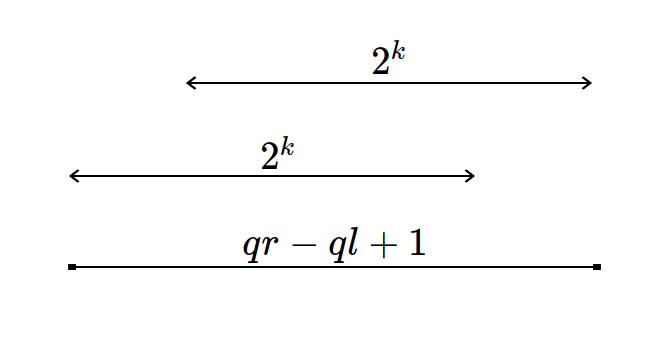
\includegraphics[width=5cm]{figures/sparse-table.png}
  \begin{itemize}
    \item 回答一個詢問 \([ql, qr]\) 最大值時,我們可以找到最大的 \(k\) 使得 \(2^k \leq qr - ql + 1\)
    \item 那麼 \([ql, qr]\) 正好可以用兩個長度 \(2^k\) 的區間的聯集湊出來!
    \item 也就是說,把序列每個位置做為開頭,長度是 $1, 2, 4, 8$ 等等 $2$ 的冪次長度的子序列的最大值存起來,就可以在 $O(1)$ 的時間回答一個詢問了
  \end{itemize}
\end{frame}

\begin{frame}{Sparse Table}
  \begin{itemize}
    \item 把序列每個位置做為開頭,長度是 $1, 2, 4, 8$ 等等 $2$ 的冪次長度的子序列的最大值存起來
    \item 看起來我們預處理的資訊有 $O(N) \times O(\log N) = O(N \log N)$ 個
    \item 令 \(f(i, j)\) 表示區間 \([i, i+2^j)\) 的最大值
    \item 也就是說,$f(i, j)$ 是從 $i$ 開始往後 $2^j$ 這個連續序列的最大值
  \end{itemize}
\end{frame}

\begin{frame}{Sparse Table}
  \begin{itemize}
    \item 把序列每個位置做為開頭,長度是 $1, 2, 4, 8$ 等等 $2$ 的冪次長度的子序列的最大值存起來
    \item 看起來我們預處理的資訊有 $O(N) \times O(\log N) = O(N \log N)$ 個
    \item 令 \(f(i, j)\) 表示區間 \([i, i+2^j)\) 的最大值
    \item 也就是說,$f(i, j)$ 是從 $i$ 開始往後 $2^j$ 這個連續序列的最大值
    \item 要怎麼更新呢?
  \end{itemize}
\end{frame}

\begin{frame}[fragile]{Spare Table}
  \begin{itemize}
    \item 
    \begin{minted}[breaklines]{cpp}
      int f[kN][klogN];
      for (int i = 0; i < kN; ++i) {
        for (int j = 0; j < klogN; ++j) {
          f[i][j] = a[i];
          for (int k = i; k < min(i + (1 << j), n); ++k) {
            f[i][j] = max(f[i][j], a[k]);
          }
        }
      }
    \end{minted}
    \item 每個預處理資料都用 $O(N)$ 算答案,複雜度為 $O(N^2 \log N)$,TLE
    \item 有辦法\textbf{重複利用已經預處理好的資料}嗎?
  \end{itemize}
\end{frame}

\begin{frame}[fragile]{Sparse Table}
  \begin{itemize}
    \item 來試試看吧!
    \item 令 \(f(i, j)\) 表示區間 \([i, i+2^j)\) 的最大值
    \item $j = 0$ 好像沒啥辦法,就是個 $f(i, 0) = a_i$
    \item $j = 1$ 呢?好像就是 $f(i, 1) = \max(a_i, a_{i + 1})$,還看不太出來
    \item $j = 2$ 呢? $f(i, 2) = \max(\{a_i, a_{i + 1}, a_{i + 2}, a_{i + 3}\})$
    \item 試著對半切切看呢?$f(i, 2) = \max(\max(a_i, a_{i + 1}), \max(a_{i + 2, i + 3}))$
    \item 咦,$\max(a_i, a_{i + 1})$ 好像是 $f(i, 1)$ 耶,$\max(a_{i + 2}, a_{i + 3})$ 好像是 $f(i + 2, 1)$
    \item 長度是 $4$ 可以被拆成 $2 + 2$!
  \end{itemize}
\end{frame}

\begin{frame}[fragile]{Sparse Table}
  \begin{itemize}
    \item 令 \(f(i, j)\) 表示區間 \([i, i+2^j)\) 的最大值
    \item 所以其實,$j = 1$ 的 $f(i, 1) = \max(a_i, a_{i + 1})$ 也可以寫成 $f(i, 1) = \max(f(i, 0), f(i + 1, 0))$
    \item 所以,假設我們已經有所有長度是 $1$ 的答案了(就是 $a$ 序列本身)
    \item 我們就會有長度是 $2$ 的答案(每個長度是 $2$ 的答案都可以由 $1 + 1$ 組出來)
    \item 我們就會有長度是 $4$ 的答案(每個長度是 $4$ 的答案都可以由 $2 + 2$ 組出來)
  \end{itemize}
\end{frame}

\begin{frame}{Sparse Table}
  \begin{itemize}
    \item 令 \(f(i, j)\) 表示區間 \([i, i+2^j)\) 的最大值
    \item 所以,比較大方向的來說,長度是 $2^j$ 的區間可以由兩個長度對半($2^{j - 1}$)區間的答案湊出來
    \item 第一段的開頭是 $i$,第二段的開頭是 $i + 2^{j - 1}$
    \item $f(i, j) = \max(f(i, j - 1), f(i + 2^{j - 1}, j - 1))$
    \item 這個更新的式子是 $O(1)$ 的!也就是說,更新一個預處理資料為 $O(1)$
    \item 預處理的複雜度為 $O(N \log N) \times O(1) = O(N \log N)$
    \item \(\langle {O}(N \log N), {O}(1)\rangle\)
  \end{itemize}
\end{frame}

\begin{frame}[fragile]{\btitle{範例實作}}
  \begin{minted}[breaklines]{cpp}
    for (int i = 0; i < n; i++)
      mx[0][i] = arr[i];
    for (int lg = 0; lg + 1 < maxlg; lg++) {
      int len = 1 << lg;
      for (int i = 0; i + len < n; i++) // 注意 i + len 不要超出邊界
        mx[lg + 1][i] = std::max(mx[lg][i], mx[lg][i + len]);
    }
  \end{minted}
\end{frame}

\begin{frame}[fragile]{\btitle{範例實作}}
  \begin{minted}[breaklines]{cpp}
    int query(int l, int r) { // returns max([l, r])
      int lg = std::__lg(r - l + 1);
      int len = 1 << lg;
      return std::max(mx[lg][l], mx[lg][r - 1 - len]);
    }
  \end{minted}

  \texttt{std::\_\_lg()} 這個函數會回傳該數字以 $2$ 為底的對數的整數部份,速度比正常的 \texttt{log2()} 快上許多
\end{frame}

\begin{frame}[fragile]{\btitle{總結}}
  \begin{itemize}
    \item $O(N \log N)$ 預處理,$O(1)$ 查詢
    \item \textbf{不能支援修改}
    \item 可以用在\textbf{重複取不會對答案造成影響的詢問},比如說 gcd、bitwise-and/or
    \item 詢問很多的話可以派上用場!
    \item 思考:為什麼要用 $2^n$ 劃分,用 $3^n$ 不好嗎?
  \end{itemize}
\end{frame}

\end{document}
